\begin{figure}[h]
  \centering
  
  
   \begin{subfigure}{0.49\linewidth}
  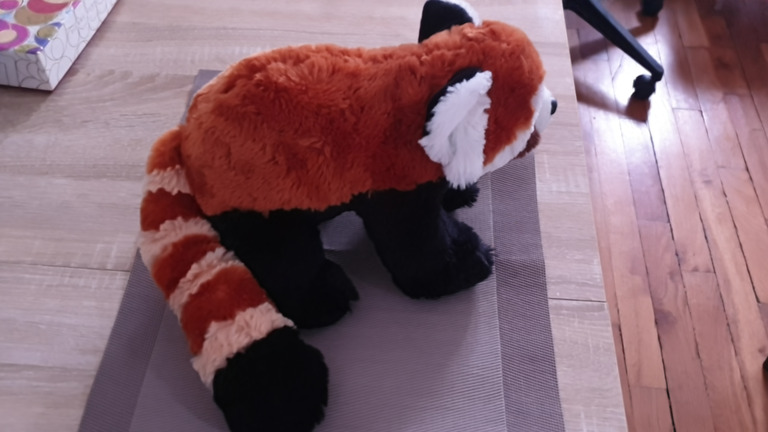
\includegraphics[width=0.99\linewidth]{images/renders/panda1_rgb_166.jpg}
  \caption{Rendering}
  \end{subfigure}
  \hfill
  \begin{subfigure}{0.49\linewidth}
  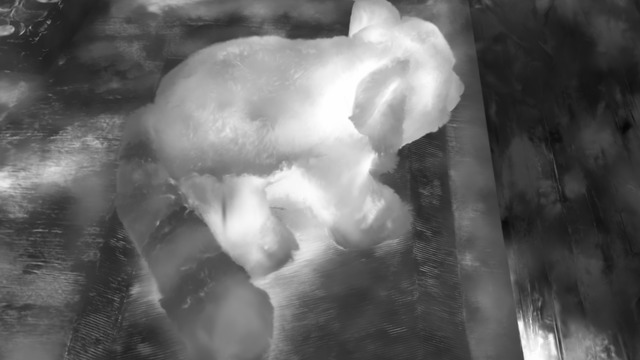
\includegraphics[width=0.99\linewidth]{images/frosting_size/panda1_size_166.jpg}
  \caption{Thickness of the Frosting layer}
  \end{subfigure}
  
  % 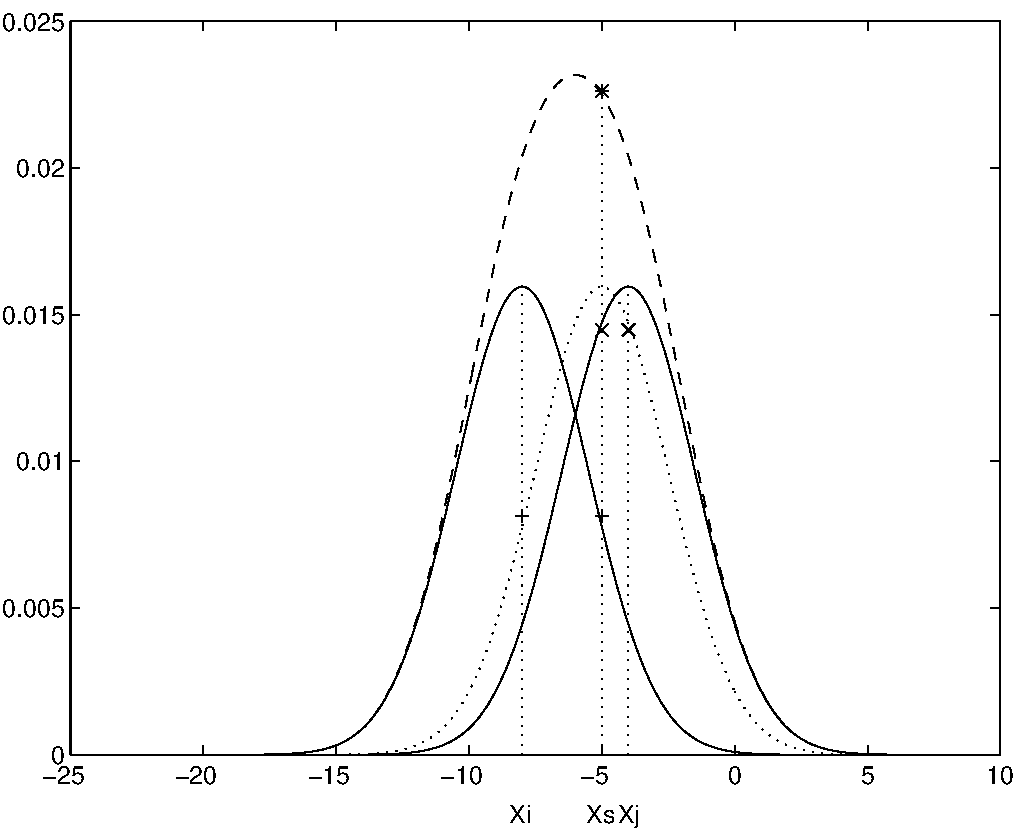
\includegraphics[height=6.5cm]{eijkel2}
  % \fbox{\rule{0pt}{2in} \rule{.9\linewidth}{0pt}}
  \caption{
  % We propose to represent surfaces by a mesh covered with a ``frosting'' layer of varying thickness and made of 3D Gaussians. This representation captures both complex volumetric effects created by fuzzy materials such as the cat's hair as well as flat surfaces. It can be rendered in real-time and animated using traditional animation tools as shown in the video provided as supplementary material. We also propose a method to build this representation from color images and capture fine details as seen in the rendered image and the normal map.
  \textbf{Visualization of the thickness of the Frosting layer on an example.} A thicker layer is shown with a brighter value. Our method automatically builds a thick Frosting layer for fuzzy areas  such as the fur of the red panda plush, and a thin Frosting layer for flat surfaces such as the table or the floor. Adapting the thickness of the Frosting layer allows for allocating more Gaussians in areas where more volumetric rendering is necessary near the surface, resulting in an efficient distribution of Gaussians in the scene. As we demonstrate in the paper, using an adaptive thickness results in higher performance than using a predefined constant thickness, and reduces artifacts when animating the mesh.}
  \label{fig:teaser}
\end{figure}